\documentclass{sig-alternate}

\usepackage[utf8]{inputenc}
\usepackage[activate=compatibility]{microtype}

% autoref command
\usepackage[hyphens]{url}
\usepackage[pdftex,urlcolor=black,colorlinks=true,linkcolor=black,citecolor=black]{hyperref}
\def\sectionautorefname{Section}
\def\subsectionautorefname{Subsection}
\def\subfigureautorefname{Subfigure}

\usepackage{setspace}

% Graphics
\usepackage{graphicx}
\usepackage{subfig}
\usepackage[font=small]{caption}
\captionsetup[figure]{name=Figure}
\usepackage{subcaption}

\usepackage{amsmath}
\usepackage{enumitem}
\usepackage{pbox}
\usepackage{color}
\definecolor{light-gray}{gray}{0.8}

% todo macro
\usepackage{color}
\newcommand{\todo}[1]{\noindent\textcolor{red}{{\bf \{TODO}: #1{\bf \}}}}

% listings and Verbatim environment
\usepackage{fancyvrb}
\usepackage{relsize}
\usepackage{listings}
\usepackage{verbatim}
\newcommand{\defaultlistingsize}{\fontsize{8pt}{9.5pt}}
\newcommand{\inlinelistingsize}{\fontsize{8pt}{11pt}}
\newcommand{\smalllistingsize}{\fontsize{7.5pt}{9.5pt}}
\newcommand{\listingsize}{\defaultlistingsize}
\RecustomVerbatimCommand{\Verb}{Verb}{fontsize=\inlinelistingsize}
\RecustomVerbatimEnvironment{Verbatim}{Verbatim}{fontsize=\defaultlistingsize}
\lstset{frame=lines,captionpos=b,numberbychapter=false,escapechar=§,
        aboveskip=2em,belowskip=1em,abovecaptionskip=0.5em,belowcaptionskip=0.5em,
        framexbottommargin=-1em,basicstyle=\ttfamily\listingsize\selectfont}

% use Courier from this point onward
\let\oldttdefault\ttdefault
\renewcommand{\ttdefault}{pcr}
\let\oldurl\url
\renewcommand{\url}[1]{\inlinelistingsize\oldurl{#1}}

\lstdefinelanguage{JavaScript}{
  keywords={push, typeof, new, true, false, catch, function, return, null, catch, switch, var, if, in, while, do, else, case, break},
  keywordstyle=\bfseries,
  ndkeywords={class, export, boolean, throw, implements, import, this},
  ndkeywordstyle=\color{darkgray}\bfseries,
  identifierstyle=\color{black},
  sensitive=false,
  comment=[l]{//},
  morecomment=[s]{/*}{*/},
  commentstyle=\color{darkgray},
  stringstyle=\color{red},
  morestring=[b]',
  morestring=[b]"
}

% linewrap symbol
\definecolor{grey}{RGB}{130,130,130}
\newcommand{\linewrap}{\raisebox{-.6ex}{\textcolor{grey}{$\hookleftarrow$}}}

\hyphenation{WebGL}

\begin{document}

\title{Analytics of Realtime Soccer Match Sensor Data with JavaScript and WebGL---Reprocessed and Visualized for Web Browser or Command Line Consumption}

\numberofauthors{1}\author{
\alignauthor
Martin Kleppe\\
  \affaddr{Ubilabs GmbH}\\
  \affaddr{Juliusstr. 25}\\
  \affaddr{22769 Hamburg, Germany}\\
  \email{kleppe@ubilabs.net}
}
\maketitle

\begin{abstract}
In this paper, we report on a~Web application 
with an additional command line interface
capable of providing complex analyses
over high velocity soccer match sensor data
that was implemented in JavaScript
and the Web Graphics Library~(WebGL).
This application visualizes analysis results graphically
in the Web browser and in parallel also
streams aggregated statistics in realtime
to a~command line interface.
The data analyzed in this paper consists of raw sensor data
that was recorded during an actual soccer match
using wireless sensors embedded in the ball
and the players' shoes.
The thereof generated realtime analyses are twofold:
on the one hand, they focus on the continuous computation of statistics
such as ball possession, shots on goal, or player of the match,
which is relevant to passive spectators like fans in a~stadium
or TV viewers at home.
On the other hand, they focus on active observers of the match
like team coaches or team managers that require more detailed analyses
like running path visualizations, position heatmaps, \emph{etc.}
\end{abstract}

\keywords{Realtime Analyses, Sensor Data, Data Streams, JavaScript, WebGL, Command Line Interface, Sports, Soccer}

\section{Introduction}

Detailed sports game analyses are of high interest and
relevance in today's professional sports leagues.
Spectators are provided with additional statistics
such as the number of shots on the goal, movement analyses,
or percentage of ball possession per player or team.
Furthermore, more detailed statistics provide useful information
for coaches and team managers about players' performance
during the match or in certain situations
and also give insights about opponents,
which could lead to modification in tactics.
Although automated solutions
such as high resolution video analyses are desirable
as they generate the required detailed statistics quickly,
at present, most sports game statistics are still processed manually.
Unfortunately, insights gained through image-based solutions
are limited by image resolution, frame rate, and last not least
prohibitive costs.
For the ACM DEBS~2013 Grand Challenge,%
\footnote{DEBS Challenge: \url{http://www.orgs.ttu.edu/debs2013/}}
the Fraunhofer Institute for Integrated Circuits~(IIS)%
\footnote{Fraunhofer IIS \url{http://www.iis.fraunhofer.de/}}
have set up a~realtime locating system on a~soccer field
in a~stadium in Nuremberg, Germany.
Every player and the ball were equipped with wireless sensors
that produce high velocity sensor data at a~total rate
of about 15,000 position events per second.

In the following, we will outline our submission to the challenge
that uses continuous computation of statistics in JavaScript
to generate interactive visualizations and realtime analyses
of the game such as ball possession, shots on goal,
running analyses of all players and the two teams.
The chosen approach can be called \emph{hybrid},
as the same system is used to visualize the game in a~Web browser%
\footnote{We have tested our application in Google Chrome, version~26 for Mac~OS~X: \url{https://www.google.com/chrome}}
and to output multiple event streams on the file system.

A~short screencast of our application is available online 
at \url{http://bit.ly/debs-challenge-video} and the source code
of our challenge contribution can be found on GitHub at
the URL \url{https://github.com/ubilabs/soccer-debs-challenge/}.

The remainder of this paper is structured as follows.
We cover related work in \autoref{sec:related-work}.
In \autoref{sec:methodology}, we outline
the methodology we used to approach the challenge problems.
\autoref{sec:implementation-details}
is dedicated to implementation details and performance optimizations.
We conclude with an outlook on future work in \autoref{sec:conclusions-future-work}.

\section{Related Work}
\label{sec:related-work}

Automated sport analyses heavily depend on video systems
that capture the game, compute differences between images
and then use the remaining color information
to track players and ball%
~\cite{Huang:2007:PBD:1776594.1776646,Liang:2005:SBD:2163110.2163186}.
Another approach is to equip the players with sensors
that collect position data over time.
This data can be combined with video processing,
which can serve, for example,
to select and zoom in on a~situation where a~certain player
is within the opponent's penalty area~\cite{ragnar2012football}.
Additionally, biometric sensors that collect information
about the players' conditions---such as heartbeats
and body temperatures---provide data that is used
to analyze the performance during the game~%
\cite{alonso2010sportstelemetry}.
Spatial game analytics (\emph{e.g.}, heatmaps
that display the players' distribution over time)
are widely recognized by sports professionals
as one of the most useful applications,
because they can be used to optimize the team distribution
for a~specific game~\cite{elnasr2013spatialgame}.

Using JavaScript to analyze enormous amounts of data in realtime---%
as it is the case with high accuracy sensory data---%
was not possible until Node.js,%
\footnote{Node.js: \url{http://nodejs.org/}}
a server-side software system designed for
writing scalable Internet applications, notably Web servers.
Node.js programs are written on the server side
in JavaScript, using event-driven, asynchronous I/O
to minimize overhead and maximize scalability.
Node.js is a~packaged compilation of Google's V8 JavaScript engine%
\footnote{V8: \url{https://code.google.com/p/v8/}}
and was shown to be suitable for building
high-performance network programs%
~\cite{tilkov2010node}
thanks to its event-driven and non-blocking nature.
Furthermore, HTML5 features such as Canvas and WebSockets
are used for realtime monitoring systems%
~\cite{cha2013developing}.

When visualizing three-dimensional content,
WebGL~\cite{webgl},%
\footnote{WebGL: \url{http://webgl.org/}}
a Web standard for a~low-level 3D graphics API
based on OpenGL ES 2.0,%
\footnote{OpenGL: \url{http://www.khronos.org/opengles/2_X/}}
is the tool of choice to render 3D objects
in the browser.
It is used for MMOGs (Massively Multiplayer Online Games)%
~\cite{chenwebgl},
efficient rendering of 3D models%
~\cite{sawicki2013efficient},
and interactive visualization of volumetric data%
~\cite{congote2011interactive}.

\section{Problem Approach}
\label{sec:methodology}

Our present submission to the ACM DEBS 2013 Grand Challenge
started with the question: ``is it possible to read and analyze
the provided input data stream and visualize it in the browser?''
In a~first step, initial tests turned out that
parsing the provided file with the raw sensor data
and simply displaying the positions of all players
and balls in 3D is possible with a~factor of twenty times of the actual speed on a~standard consumer laptop,
\emph{i.e.}, a~minute of the real game is replayed
within just three seconds.
This leaves enough time to make additional calculations.
The two teams and the ball can easily rendered recognizable
by using different colors for each.
Additionally, the soccer field and goals are drawn
to visually check different game situation.

In a~second step, we implemented the required queries.
For every piece of information, a~visual element was added
to the browser interface to keep track of the computations
and avoid gross errors.
These visual elements include:
a tracing line to highlight the direction of the ball movement,  
the list of players with statistics about ball possession,
colored sparklines for running analyses,
the precalculated ball path, the potential hit target,
highlighting of the current player,
an animated acceleration bar,
and the current time.
A~screenshot of the application can be seen in
\autoref{fig:screenshot}.

In a~third step, as the application has to deal with large datasets,
it is critical to observe the internally used memory.
The Chrome Developer Tools Timeline panel%
\footnote{Chrome Developer Tools: \url{https://developers.google.com/chrome-developer-tools/docs/timeline}}
was used
to detect if any of the involved scripts
result in increasing memory usage without freeing it at the script's end.
If such memory leaks were detected, they were carefully evaluated and the memory-leaking code improved.

In a~final step, after all visual parts were included,
the original code was extended to also run
via the command line without the need of a~Web browser.
Therefore, a~bridge was created to either render HTML
or output several file streams if executed on the command line.
The result is an application that does both,
visualize the match in a~browser or store aggregated results
on the hard disk.

\begin{figure*}[t!]
  \centering
  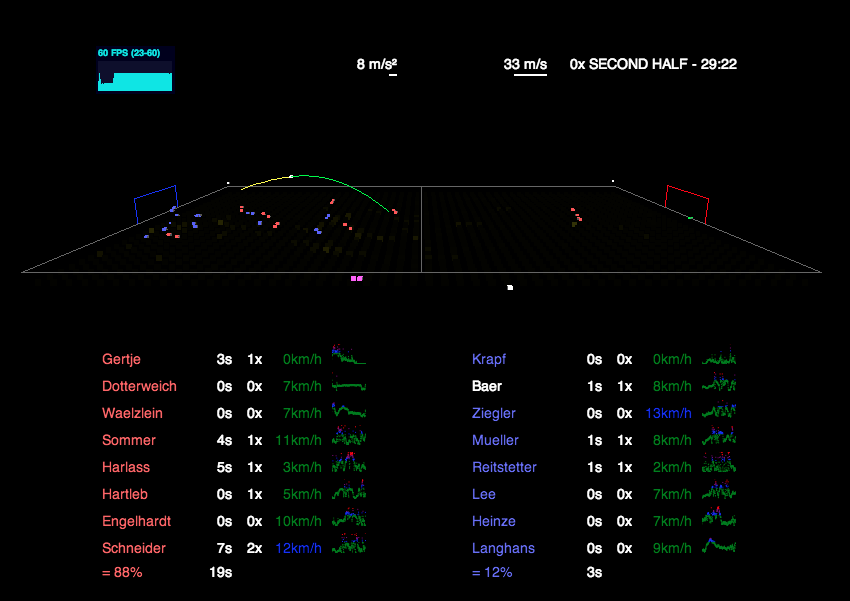
\includegraphics[width=\linewidth]{soccer.png}
  \caption{Screenshot of the application with a~tracing line to highlight the direction of the ball movement (yellow),
the precalculated ball path (green),  
the list of players with individual statistics about ball possession,
colored sparklines for running analyses, the potential hit target,
current player highlighting,
animated acceleration bar,
and current time}
  \label{fig:screenshot}
\end{figure*}

\section{Implementation Details}
\label{sec:implementation-details}

\paragraph{Input Data Format}

The original data stream was captured during the game
and resulted in a~4.62 GB CSV input file.
Position updates for sensors in players' shoes
and goalkeepers' hands are provided with a~frequency of 200Hz.
The sensors in all balls update with 2000Hz.
A~sensor record contains the following data:
sensor id, timestamp in picoseconds, position
(in a~three-dimensional coordinate system) of the sensor
in millimeters, |v| (in $\mu$m/s), vx, vy, vz
describe the speed of the direction of objects as a~vector,
and |a| (in $\mu$m/s$^{2}$), ax, ay, az describe the absolute acceleration
and its constituents in three dimensions.

\paragraph{Implemented Queries}

Based on this data, the following queries are required
for the ACM DEBS 2013 Grand Challenge:
running analysis, ball possession, heatmaps, and shots on goal.
Furthermore, goal detection and detection of when the ball is out were implemented as additional features of the application.

\paragraph{Data Flow}

All entries of the original data stream are distributed
to several JavaScript objects based on a~mapping table
that includes more information about the sensor type.
Whenever a~ball position update was detected,
the system uses the last known position to check
for a~goal or whether the ball has left the field.
If the ball acceleration peaks, it detects the associated player
and computes the shot target
based on the current speed vector and gravity.
Position updates for all players are collected
for the purpose of running statistics and heatmap calculations.

\paragraph{Performance Tuning}

To optimize performance
and to avoid long running scripts,
plain JavaScript with almost zero dependencies was used,
with the exception of the already highly performance-optimized libraries fishbone.js%
\footnote{Fishbone.js: \url{https://github.com/aemkei/fishbone.js}}
and Three.js;%
\footnote{Three.js: \url{http://threejs.org/}}
the former being an extremely lightweight JavaScript library with automatic method chaining, automatic context binding, event support, and simple inheritance and the latter being a~wrapper for low-level WebGL instructions.
The code was organized in two kinds of modules:
\emph{(i)} simple class-like modules with prototype-based inheritance
that were used for fast-changing game objects
like players or ball on the one hand
and \emph{(ii)} modules that handle events between these objects
and the streams on the other.
A~centralized runner script handles
most of the time-consuming calculations within a~flat lexical scope
to avoid nested functions and variable lookups.
This was especially critical for large loops
that occur when the input stream emits new records.

\paragraph{Data Aggregation}

Whenever an update of one of the (several during the match utilized) balls is detected,
the program evaluates if the current ball also is the currently active match ball
by comparing its position with the field's boundaries.
Then the nearest player is selected
and if the ball's acceleration peaks,
shots on goal and ball possessions
(per player and team) are evaluated.
With a~frequency of 50Hz, the player's current position
is recorded into a~large array to generate running statistics
and heatmaps based on different time frames
(1, 5, 20 minutes and the whole game).
This is done by looping through the records
multiple times per interval
and comparing all dimensions to create aggregated values.

\paragraph{Visualization}

To visualize the results in the browser,
position properties of JavaScript objects are updated
whenever new data arrives.
As WebGL is a~state machine%
~\cite{cantor2012webgl},
these updates are handled very fast.
Geometries for sensors are displayed as colored cubes,
the field and ball paths are simple polylines
and the heatmap is a~particle system.
We use rectangular sprites, as the rendering performance
of 2D sprites is considerably better than updating complex geometries%
~\cite{hoetzlein2012graphics}.
The list of players is drawn as an unordered HTML list (\texttt{<ul>})
and colors are assigned via CSS.%
\footnote{CSS: \url{http://www.w3.org/Style/CSS/}}
The color-coded sparkline graphs at the end of each list item
are drawn using HTML5 Canvas,%
\footnote{HTML5 Canvas: \url{https://dev.w3.org/html5/2dcontext}},
which was shown to perform better than plain HTML,
SVG, and WebGL, as it generates highly optimized stateless bitmaps.

\paragraph{Command Line Output}

Output for the command-line version was implemented
using so-called file streams: for every calculation that emits events,
a writable stream%
\footnote{Node.js Writable Stream: \url{http://nodejs.org/api/all.html\#all_class_stream_writable}}
is created in Node.js.
The current implementation pipes the output to multiple files
on the hard disk, each for every query type:
Player running analysis (1 stream),
aggregated running statistics (4 time frames),
player ball possession (1 stream),
team ball possession (1 stream),
heatmaps (4 time frames), and shots on goals (1 stream).
This results in a~total of 12 files written to disk.
The complete calculation of the entire match data
takes about 600 seconds on our testing device.

\section{Conclusions and Future Work}
\label{sec:conclusions-future-work}

In this paper, we have shown
that modern JavaScript engines such as V8
are well suited to process large amounts of data in realtime.
With the current two-fold implementation, it is possible to analyze a~full soccer match
on the command line and to visualize it in the browser.
HTML5 features such as Canvas and WebGL draw graphics
without any noticeable performance degradation,
and the event-driven, non-blocking I/O model of Node.js
was shown to be an efficient way to read, process, and write data.
As mentioned above, the current implementation
outputs all streams to the file system.
However, using the abstract stream pattern in Node.js,
they can be piped%
~\cite{ogden2012nodestreams}
to other types of streams such as WebSockets.%
\footnote{WebSockets: \url{http://dev.w3.org/html5/websockets/}}

In the future, this will enable the new use case of
allowing for  mobile devices such as cell phones and tablets
with limited storage
and computing power to be used for the visualization.
They connect to the main server via a~WebSocket connection
and receive only small chunks of data that are necessary
to render relevant information.
Coaches and team members can benefit from such a~solution
for mobile devices, as they are small and portable
compared to laptop computers.
Further future work can include to port the current version of the application
to other ball team sports, \emph{e.g.}, American football,
rugby or basketball.
More automatic analyses can be integrated,
such as number of corner shots, passes, and duel statistics.
If combined with additional biometric sensor data (pulse, power)
this could give insights into the current player's condition
or even training progress during a~whole season.

\section*{Acknowledgments}
We would like to thank the following persons for their valuable comments: Thomas Steiner, Nenad Nikolić, Klaus Trainer, Michael Pletziger, Jens Wille, Samuel Oey, Robert Katzki, Astrid Schildkopf.

\balancecolumns
\bibliographystyle{abbrv}
\bibliography{soccer-debs-challenge}

\end{document}